% !TEX root = ../dg.tex

\section{Manifolds and Maps}

The title of this course is ``Introduction to Differential Manifolds,'' which suggests that these \emph{differential manifolds} (or sometimes \emph{differentiable manifolds}), whatever they are, will probably be important. So what is a differential manifold? The name should suggest the answer: they are spaces in which we know what differentiation is supposed to mean. I actually prefer the term \emph{smooth manifold}, so that is what I will use going forward, though this will often just get shortened to \emph{manifold}.

In practice, the idea is to leverage the fact that we already (hopefully!) know how to do calculus in $\R^n$ (this is exactly what MATH 261 is all about), and to translate those techniques to more general spaces. The key insight here is that differentiation is a local operation: to compute a derivative at a point (whether it's a gradient, curl, divergence, directional derivative, whatever), you really only need to know what's going on in a tiny open neighborhood of that point. 

So to get a space on which we can compute derivatives, it's enough to have a space which is ``locally Euclidean'' or ``locally like $\R^n$,'' and this is what manifolds are. Roughly speaking, this means that around any point in a manifold you can find a small open set which looks just like an open set in some $\R^n$, and then we can do calculus on the manifold by translating in a neighborhood of a point to the corresponding set in $\R^n$, where we know what to do.

This is all to say that the point of defining manifolds in the way we are about to (which is extremely non-obvious and unintuitive!) is that these are precisely the spaces in which a suitable generalization of multivariable calculus makes sense.

So what does ``locally like $\R^n$'' actually mean? Here's a standard definition:

\begin{definition}\label{def:manifold}
	A \emph{smooth manifold of dimension $n$} is a Hausdorff, second-countable topological space $M$ together with a family of injective maps $\phi_\alpha\from U_\alpha \to M$ from open sets $U_\alpha \subseteq \R^n$ so that:
	\begin{enumerate}
		\item \label{it:manifold def cover}$\bigcup_\alpha \phi_\alpha(U_\alpha) = M$ (that is, the images of the maps $\phi_\alpha$ cover all of $M$);
		\item \label{it:manifold def overlap}For any $\alpha, \beta$ so that $\phi_\alpha(U_\alpha) \cap \phi_\beta(U_\beta) = W \neq \emptyset$, the sets $\phi_\alpha^{-1}(W)$ and $\phi_\beta^{-1}(W)$ are open sets in $\R^n$ and the maps $\phi_\beta^{-1} \circ \phi_\alpha$ and $\phi_\alpha^{-1} \circ \phi_\beta$ (when restricted to these open sets) are smooth.
		\item \label{it:manifold def maximal}The family $\{(U_\alpha, \phi_\alpha)\}$ is maximal with respect to \Cref{it:manifold def cover,it:manifold def overlap}.
	\end{enumerate}
	The pairs $(U_\alpha, \phi_\alpha)$ are called \emph{coordinate charts} and the (maximal) collection $\{(U_\alpha, \phi_\alpha)\}$ is called an \emph{atlas}.	
\end{definition}

See \cref{fig:chart} for a visualization of \ref{it:manifold def overlap}, showing the map $\phi_\beta^{-1} \circ \phi_\alpha$ from $\phi_\alpha^{-1}(W) \subseteq \R^n$ to $\phi_\beta^{-1}(W) \subseteq \R^n$.

\begin{figure}[htbp]
	\centering
		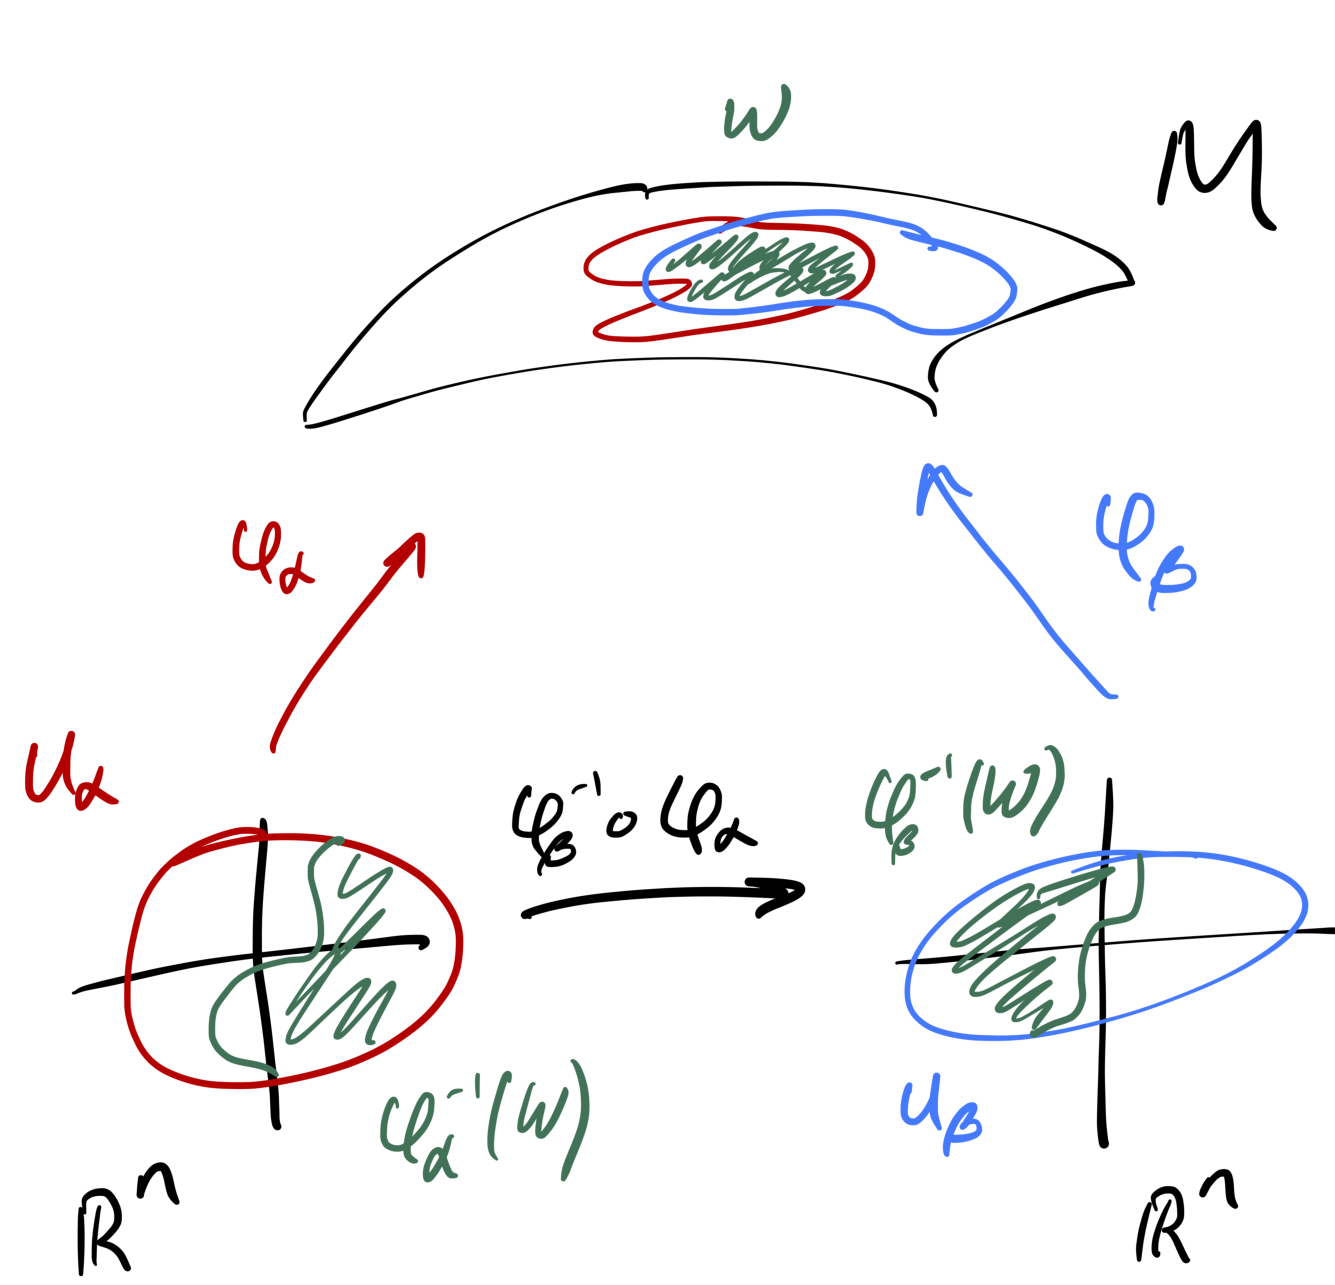
\includegraphics[height=3in]{chart}
	\caption{Transition maps.}
	\label{fig:chart}
\end{figure}

\begin{remark}
	In \ref{it:manifold def overlap} above, ``smooth'' means ``infinitely differentiable'' or, in shorthand, $C^\infty$. What I'm calling \emph{smooth manifolds} are sometimes also called $C^\infty$ \emph{manifolds}. More generally we can talk about $C^\alpha$ manifolds for any integer $\alpha \geq 0$, where we just modify \ref{it:manifold def overlap} to require the maps $\phi_\beta^{-1} \circ \phi_\alpha$ and $\phi_\alpha^{-1} \circ \phi_\beta$ to be $C^\alpha$.\footnote{Recall that a continuous map is $C^\alpha$ if it has $\alpha$ continuous derivatives.} In the special case $\alpha = 0$, this is just a requirement that these maps be continuous, and $C^0$ manifolds are often called \emph{topological manifolds}.
\end{remark}

\begin{example}
	The maximal family containing $(\R^n, \operatorname{id})$ makes $\R^n$ into a smooth manifold.
\end{example}

Of course, most interesting manifolds are not $\R^n$, but the idea of \ref{it:manifold def cover} from \cref{def:manifold} is that you can cover any manifold by a bunch of little open sets (namely, the $\phi_\alpha(U_\alpha)$) that are essentially identical to open sets in $\R^n$ (namely, the $U_\alpha$),\footnote{In topological terms, $U_\alpha$ and $\phi_\alpha(U_\alpha)$ are homeomorphic.} so you can essentially do any local calculation in $\R^n$. It's also very important that the $n$ is always the same here: if $m \neq n$, we're not allowed to have some points with neighborhoods that look like $\R^m$ and some other points whose neighborhoods look like $\R^n$.

If the idea is to use the coordinate charts to transport calculations from the manifold to $\R^n$, then a thing you should be very worried about is that, if a point lies in two different charts, then there are two different ways to do this and they might not be compatible. This is the point of \ref{it:manifold def overlap}: whether you do your calculations in $U_\alpha$ or $U_\beta$, the two are related by a smooth map, so you can easily translate between the two calculations using the change-of-variables formula. Indeed, the usual English-language gloss of \ref{it:manifold def overlap} is that ``transition functions are smooth.''

Finally, \ref{it:manifold def maximal} is a technical condition that in practice is not important. The point of it is simply to ensure uniqueness: if you had a collection of coordinate charts satisfying \ref{it:manifold def cover} and \ref{it:manifold def overlap}, and I took your collection and added some new charts while still satisfying \ref{it:manifold def overlap}, it would be kind of silly to say that you and I were talking about different manifolds. Taking maximal families gives uniqueness since your collection of charts and my collection of charts live in the same maximal family.

However, it is certainly possible to have distinct maximal collections on the same space (if there is one that is in some sense standard, then any others are sometimes called ``exotic smooth structures''). At least two Fields Medals have been awarded primarily for finding examples of exotic smooth structures: to John Milnor in 1962 (for finding exotic 7-spheres~\cite{milnorManifoldsHomeomorphic7sphere1956}; it turns out there are exactly 28 distinct smooth structures on $S^7$~\cite{kervaireGroupsHomotopySpheres1963a}) and to Simon Donaldson in 1986 (for finding exotic $\R^4$s~\cite{freedmanTopologyFourdimensionalManifolds1982,donaldsonApplicationGaugeTheory1983,gompfThreeExotic$mathbfR^4$s1983}; it turns out there are uncountably many distinct smooth structures on $\R^4$~\cite{taubesGaugeTheoryAsymptotically1987}). It remains an open problem called the \emph{smooth 4-dimensional Poincaré conjecture} whether there are non-standard differentiable structures on $S^4$.

\begin{remark}
	We often mimic the $\R^n$ notation and indicate the dimension of a manifold $M$ with a superscript; i.e., $M^n$ means that $M$ is an $n$-dimensional manifold, not that we are taking the Cartesian product $M \times M \times \dots \times M$.
\end{remark}

\begin{example}
	$S^n$ the unit sphere in $\R^{n+1}$ is a manifold. Specifically, I claim that the maximal family containing $\{(R^n, \phi_N), (R^n, \phi_S)\}$ makes $S^n$ into an $n$-dimensional manifold, where $\phi_N$ and $\phi_S$ are inverse stereographic projection from the north and south poles, respectively. 
	
	Specifically, with $\vec{x} = (x_1, \dots , x_n) \in \R^n$, define
	\[
		\phi_N(\vec{x}) := \frac{1}{1+\|\vec{x}\|^2}\left(2x_1, \dots , 2x_n, -1+\|\vec{x}\|^2\right)
	\]
	and
	\[
		\phi_S(\vec{x}) := \frac{1}{1+\|\vec{x}\|^2}\left(2x_1, \dots , 2x_n, 1-\|\vec{x}\|^2\right).
	\]
	
	Then $\phi_N$ is the map that sends $\vec{x} \in \R^n$ to the point on the sphere which lies on the line segment connecting $(x_1,\dots , x_n, 0) \in \R^{n+1}$ to the north pole $(0, \dots , 0, 1) \in S^n \subset \R^{n+1}$; see \cref{fig:stereo}. 
	
	\begin{figure}[htbp]
		\centering
			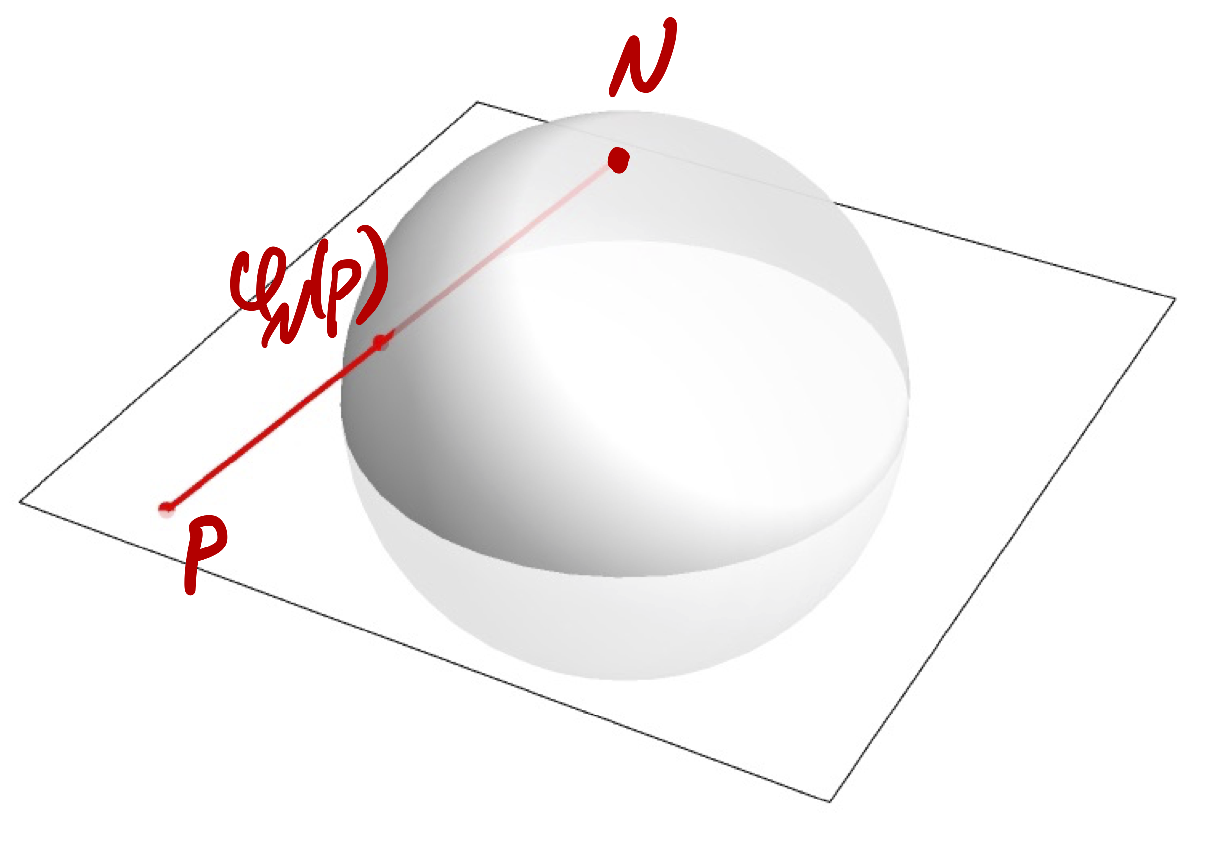
\includegraphics[height=2in]{stereo}
		\caption{Inverse stereographic projection.}
		\label{fig:stereo}
	\end{figure}

To prove the claim, we need to show that \ref{it:manifold def cover} and \ref{it:manifold def overlap} from \cref{def:manifold} are satisfied (\ref{it:manifold def maximal} is automatically satisfied, since we're taking the maximal family containing $\{(R^n, \phi_N), (R^n, \phi_S)\}$). 

If we let $N = (0,\dots , 0, 1)$ be the north pole and $S = (0,\dots , 0, -1)$ the south pole, then $\phi_N(\R^n) = S^n \backslash\{N\}$ and $\phi_S(\R^n) = S^n \backslash\{S\}$ and the union is all of $S^n$, so \ref{it:manifold def cover} is satisfied.

For \ref{it:manifold def overlap}, observe that
\[
	W = \phi_N(\R^n) \cap \phi_S(\R^n) = S^n \backslash\{N,S\},
\]
so 
\[
	\phi_N^{-1}(W) = \R^n \backslash\{0\},
\]
which is certainly open, and likewise for $\phi_S^{-1}(W) = \R^n \backslash\{0\}$. So we need to verify that $\phi_N^{-1} \circ \phi_S$ and $\phi_S^{-1} \circ \phi_N$ are smooth as functions on $\R^n \backslash\{0\}$.

The inverse of $\phi_N$ is stereographic projection 
\[
	\phi_N^{-1}(\vec{y}) := \frac{1}{1-y_{n+1}} (y_1, \dots , y_n)
\]
(check this!) so we see that
\[
	(\phi_N^{-1} \circ \phi_S)(\vec{x}) = \frac{1}{\|\vec{x}\|^2}\vec{x}
\]
is reflection through the unit sphere in $\R^n$, which is smooth away from the origin. And similarly for $\phi_S^{-1} \circ \phi_N$.
\end{example}

As already mentioned, the point of manifolds is that they are spaces in which we can do calculus, so we should be able to say what it means for a map between manifolds to be differentiable. Hopefully it's already starting to become clear what the strategy is: we can talk about differentiability at a point, and then both the point in the domain and the point it maps to in the range lie in coordinate charts that are like open sets in Euclidean spaces. So then locally our map just looks like a map between Euclidean spaces, where we already know what it means for a map to be differentiable.

\begin{definition}\label{def:differentiable}
	Let $M^m$ and $N^n$ be manifolds. A continuous map $f\from M \to N$ is \emph{differentiable} at $p \in M$ if, given a coordinate chart $\psi\from V \subseteq \R^n \to N$ containing $f(p)$, there exists a coordinate chart $\phi\from U \subseteq \R^m \to M$ containing $p$ so that $f(\phi(U)) \subseteq \psi(V)$ and 
	\[
		\psi^{-1} \circ f \circ \phi\from U \subseteq \R^m \to \R^n
	\]
	is differentiable at $\phi^{-1}(p)$ (see \cref{fig:differentiable}). The map $f$ is differentiable on an open set in $M$ if it is differentiable at every point in that set.
\end{definition}

\begin{figure}[htbp]
	\centering
		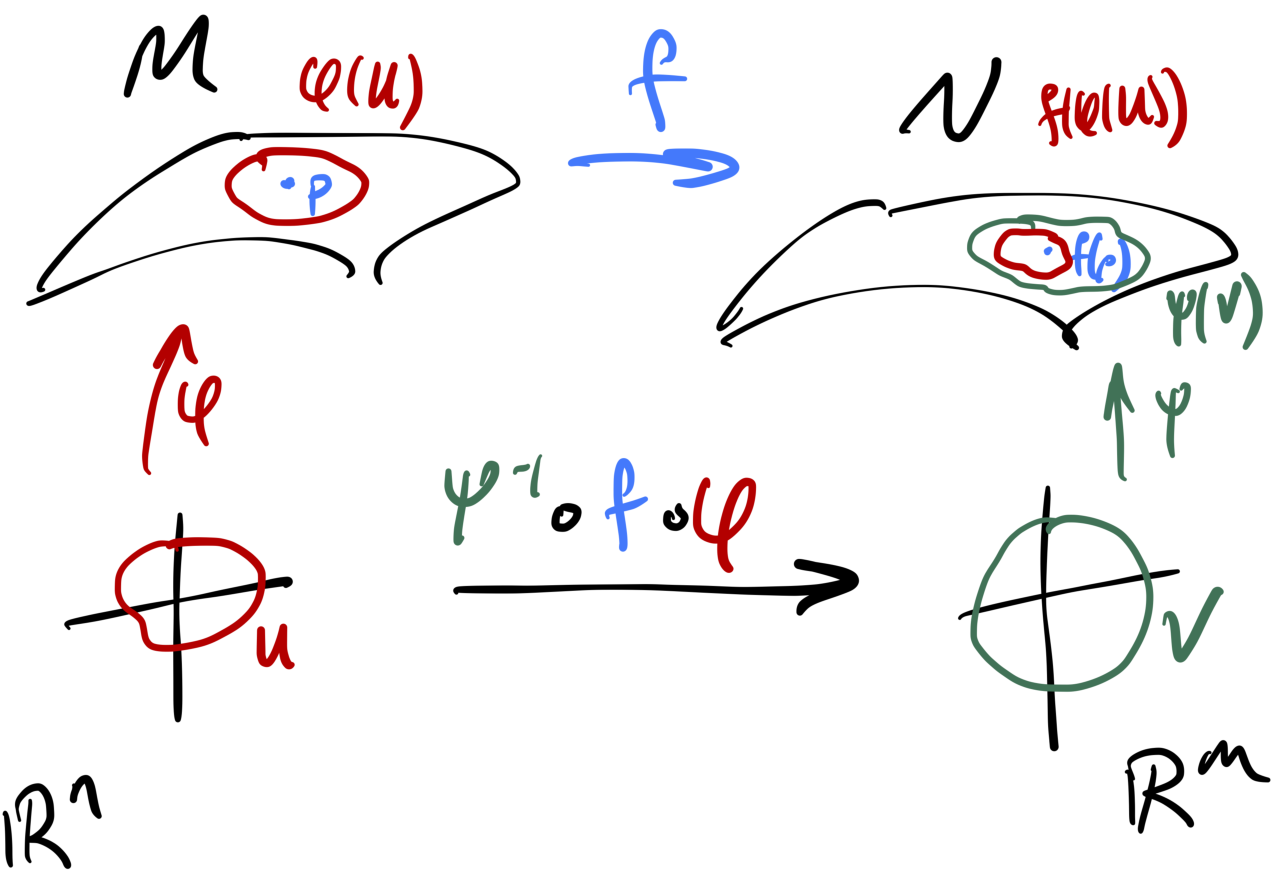
\includegraphics[height=2in]{differentiability}
	\caption{Locally converting a map between manifolds to a map between open sets in Euclidean spaces, where we know what differentiability means.}
	\label{fig:differentiable}
\end{figure}

\begin{example}
	Consider the antipodal map $\alpha : S^n \to S^n$ given by $\alpha(\vec{y}) = -\vec{y}$. Then, so long as $\vec{y}$ is not the south pole, $\alpha(\vec{y}) = -\vec{y} \in \phi_N(\R^n)$ so we can take $\psi = \phi_N$ and $V = \R^n$. Moreover, $\vec{y} \in \phi_S(\R^n)$ so we can $\phi = \phi_S$ and $U = \R^n$, since $\alpha(\phi_S(\R^n)) = S^n \backslash\{N\} = \phi_N(\R^n)$. Then a straightforward calculation shows that
	\[
		(\phi_N^{-1} \circ \alpha \circ \phi_S)(\vec{x}) = -\vec{x},
	\]
	which is definitely differentiable everywhere (as a map $\R^n \to \R^n$). 
	
	Of course, if $\vec{y} = S$, we can swap the roles of $\phi_N$ and $\phi_S$ in the above, and we conclude that $\alpha$ is differentiable everywhere on $S^n$.
\end{example}

While we've given the definition of a manifold and of a differentiable map in this section, we generally try to use them directly as little as possible. They are hard to handle and fairly unintuitive, so we will quickly be looking for alternative ways of characterizing manifolds and differentiable maps.
